\subsection*{hanging string}

\begin{center}
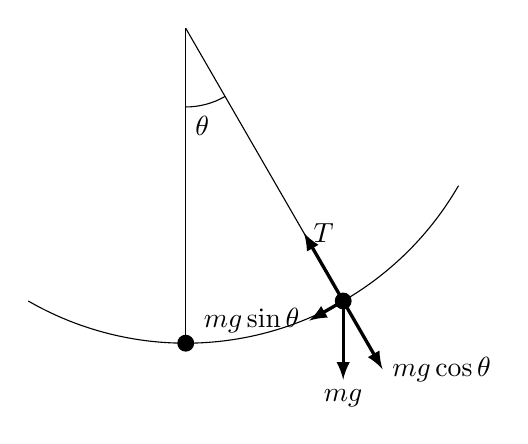
\begin{tikzpicture}

\draw (0,-4) arc [start angle=-90, end angle= -30, radius = 4] ;
\draw (0,-4) arc [start angle=-90, end angle= -120, radius = 4] ;
\draw (0,0) -- (0,-4) ;
\draw [fill] (0,-4) circle [radius=0.1] ; 
\draw [fill] (-60:4) circle [radius=0.1] ;
\draw (0,0) -- (-60:4) ;
\draw (0,-1) arc [start angle =-90, end angle=-60,radius=1] ;
\draw (0,-1) node [anchor=north west] {$\theta$} ;
\draw [very thick,-{latex}] (-60:4) -- ++(0,-1) ;
\draw (-60:4) ++(0,-1) node [anchor=north] {$mg$} ;
\draw [very thick,-{latex}] (-60:4) -- ++(-150:0.5) ;
\draw (-60:4) ++(-150:0.5) node [anchor=east] {$mg\sin\theta$} ;
\draw [very thick,-{latex}] (-60:4) -- ++(-60:1) ;
\draw (-60:4) ++(-60:1) node [anchor=west] {$mg\cos\theta$} ;
\draw [very thick,-{latex}] (-60:4) -- ++(120:1) ;
\draw (-60:4) ++(120:1) node [anchor=west] {$T$} ;

\end{tikzpicture}
\end{center}